\section{Particle Identification}\label{section:star_PIDdEdx}

The specific ionization energy loss, the $dE/dx$, is a function of magnitude of the
particle momentum. However, at the midrapidity region of $|\eta| < 0.7$, $p_\textrm{T}$ is approximately equal to $|p|$. In this section the particle identification by the $dE/dx$ at low $p_\textrm{T}$ is described.
The particle identification at high $p_\textrm{T}$ is possible
by the TOF, but due to the low particle multiplicity and lack of signal in VPDs on the outgoing proton side (presence of the rapidity gap) in SD events, the time of collision is not defined precisely enough. Therefore, the~analysis was limited to identification only by $dE/dx$. 

The ionization energy loss of charged particles in material
is given by the Bethe-Bloch formula and for
the \ac{STAR} \ac{TPC} by the more precise Bichsel formula~\cite{Bichsel:2006cs}.
The particle type can be determined by comparison of particle's $dE/dx$ with the Bethe-Bloch (Bichsel) expectations.
Figure \ref{fig:star_dedx} shows the  $dE/dx$ versus rigidity $q\times p$ for particles in $|\eta| < 0.7$. Various particles are  separated at low $|q\times p|$, whereas at higher $|q\times p|$ the $dE/dx$ of different particle species starts to
overlap: $e^\pm$ and $K^\pm$ merge at $\sim0.4$~GeV/c, $K^\pm$ and
$\pi^\pm$ merge at $\sim0.7$~GeV/c, and $p(\bar{p})$ and $\pi^\pm$ merge
at $\sim1$~GeV/c. 
\begin{figure}[h!]
	\centering
	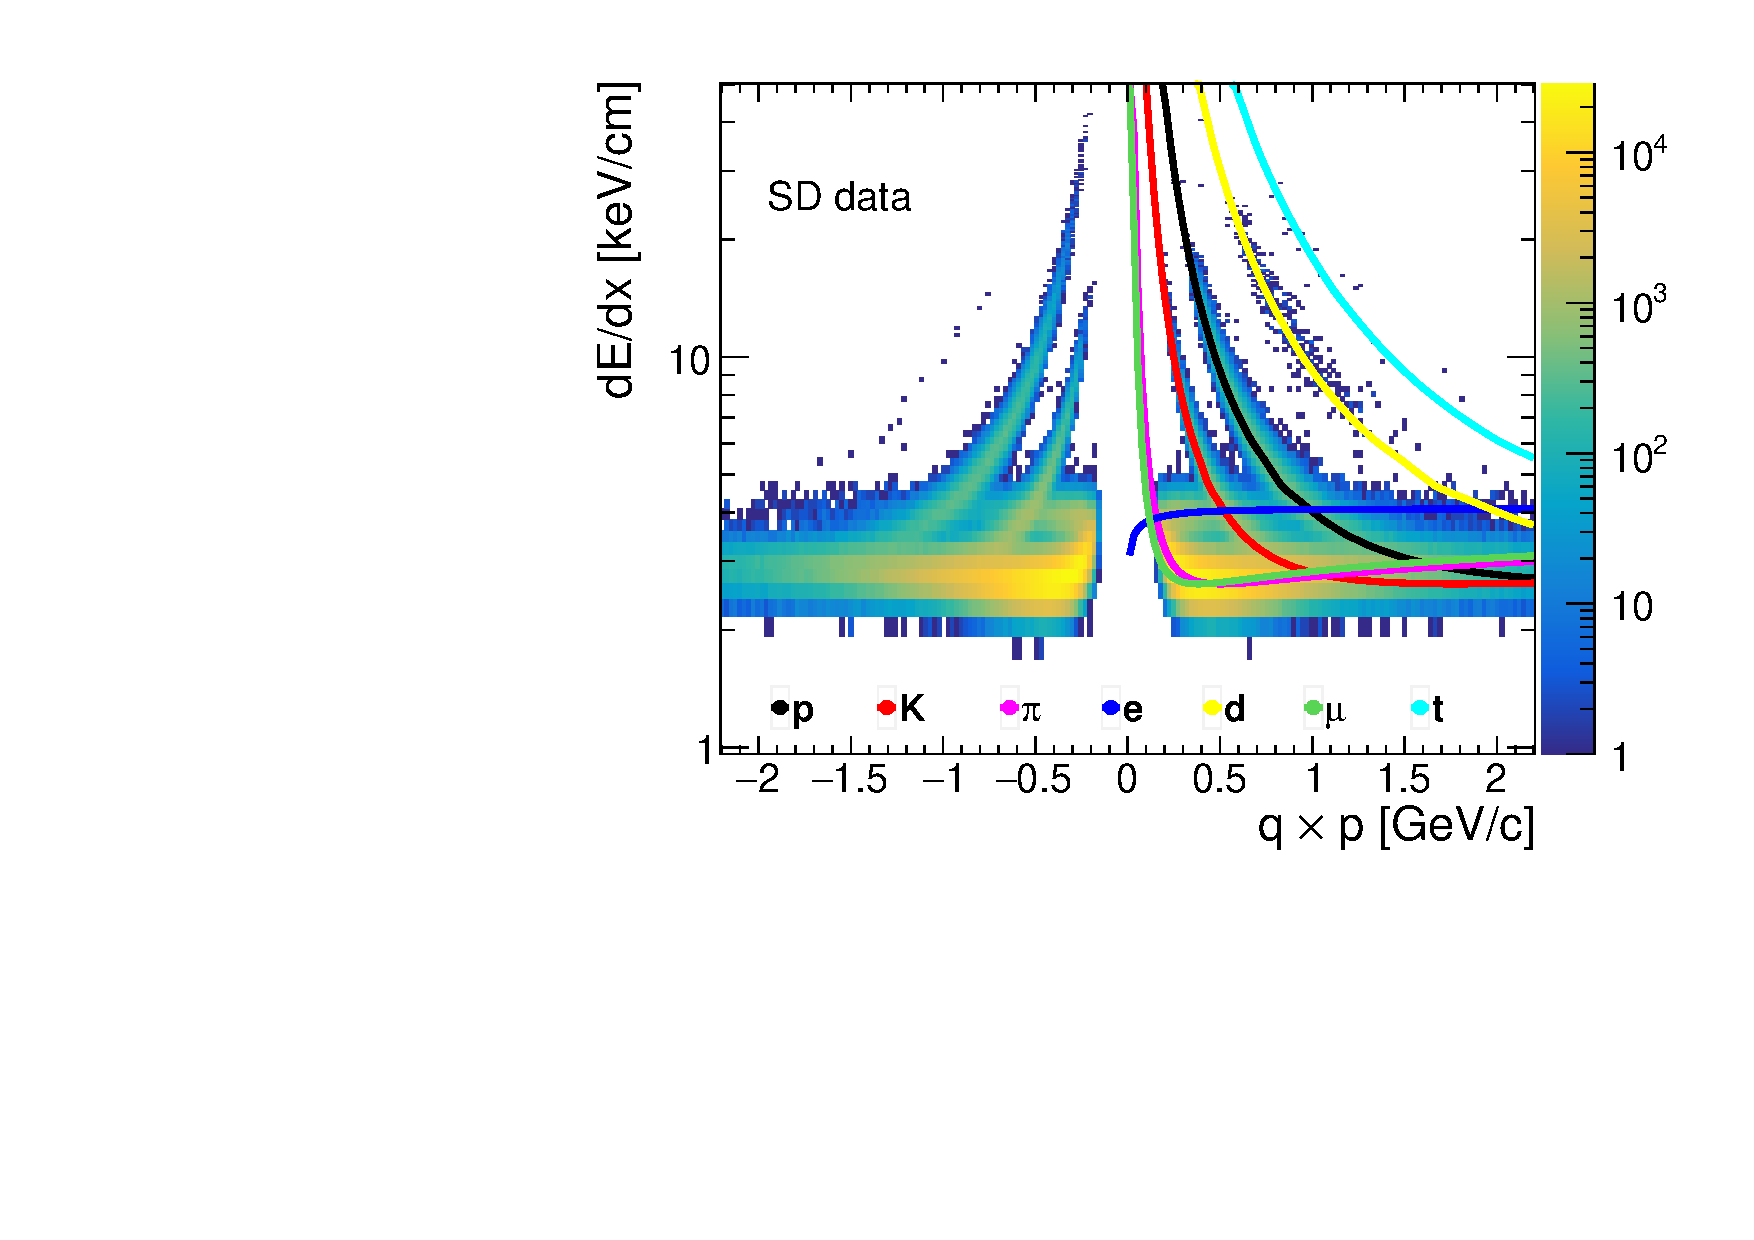
\includegraphics[width=0.8\linewidth, page=1]{chapters/chrgSTAR/img/dEdx/SDT_dEdx.pdf}
	\caption[Specific ionization
	energy loss $dE/dx$ as a function of rigidity $q\times p$ for particles
	in $|\eta| < 0.7$]{Specific ionization
		energy loss $dE/dx$ as a function of rigidity $q\times p$ for particles
		in $|\eta| < 0.7$. The Bichsel predictions for each particle species are also shown.}
	\label{fig:star_dedx}
\end{figure} 
%\FloatBarrier
\noindent Since the $dE/dx$ distribution for a fixed particle type
is not Gaussian, the following variable for each particle type was defined:
\begin{equation}
n\sigma^i_{dE/dx}=\ln\left(\frac{dE/dx}{(dE/dx)_i^\textrm{{BB}}}\right)/\sigma
\label{eq:nsigma}
\end{equation}
where $(dE/dx)_i^\textrm{{BB}}$ is the Bethe-Bloch (Bichsel) expectation
of $dE/dx$ for the given particle type $i$ $(i =
\pi, K, p)$, $\sigma$ - the $dE/dx$ resolution.
The expected value of $n\sigma^i_{dE/dx}$ for the~particle under consideration is around $0$  and the width equals to $1$. The sample $n\sigma^i_{dE/dx}$ distribution for $\pi^{\pm}$, $K^\pm$ and $p(\bar{p})$ in one $\xi$ range, $0.02 < \xi < 0.05$, is shown  in Fig.~\ref{fig:dEdx_nsigma}.
\begin{figure}[h!]
	\label{fig:dEdx_nsigma}
	\centering
	\begin{subfigure}{.49\textwidth}
		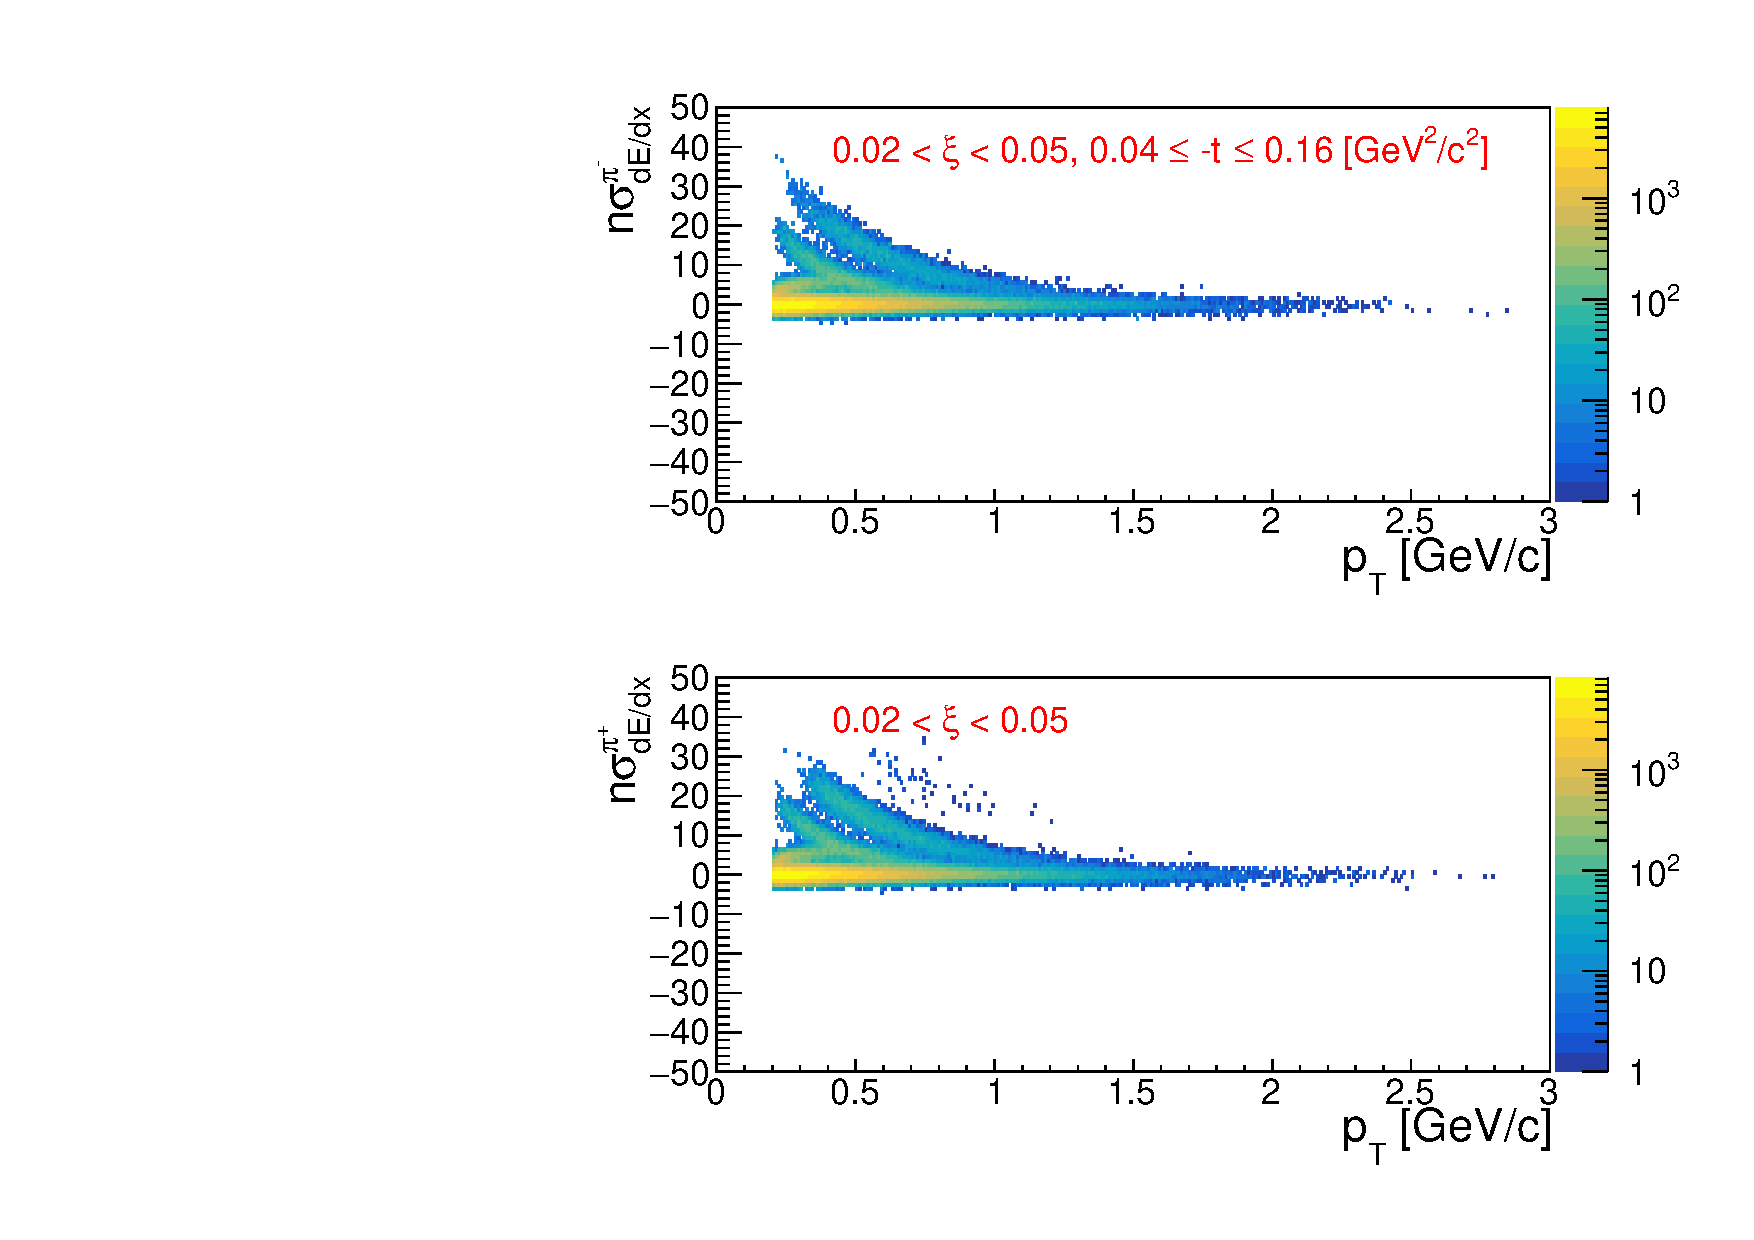
\includegraphics[width=\linewidth, page=1]{chapters/chrgSTAR/img/dEdx/fit2019_2dNsigma_0_0.pdf}
	\end{subfigure}
	\begin{subfigure}{.49\textwidth}
		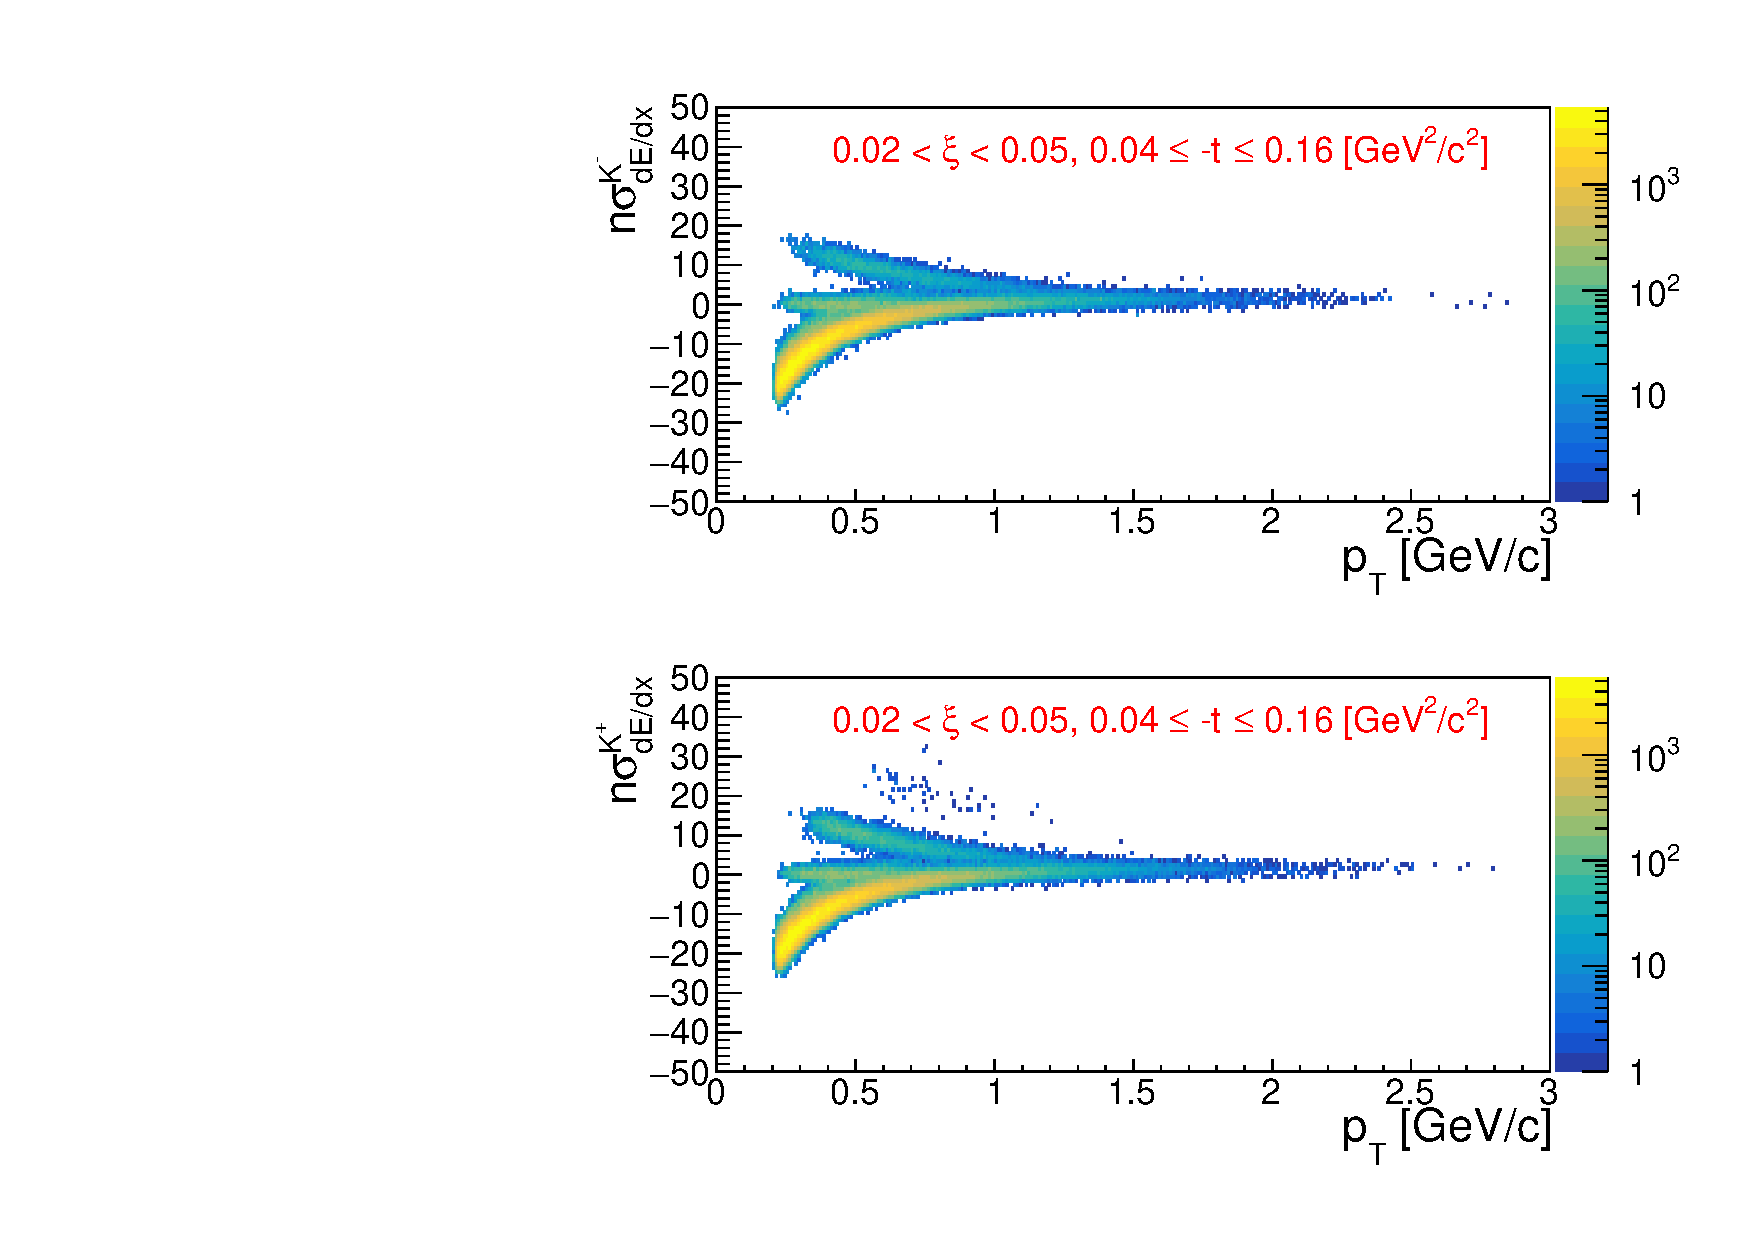
\includegraphics[width=\linewidth, page=1]{chapters/chrgSTAR/img/dEdx/fit2019_2dNsigma_0_1.pdf}
	\end{subfigure}
	\begin{subfigure}{.49\textwidth}
		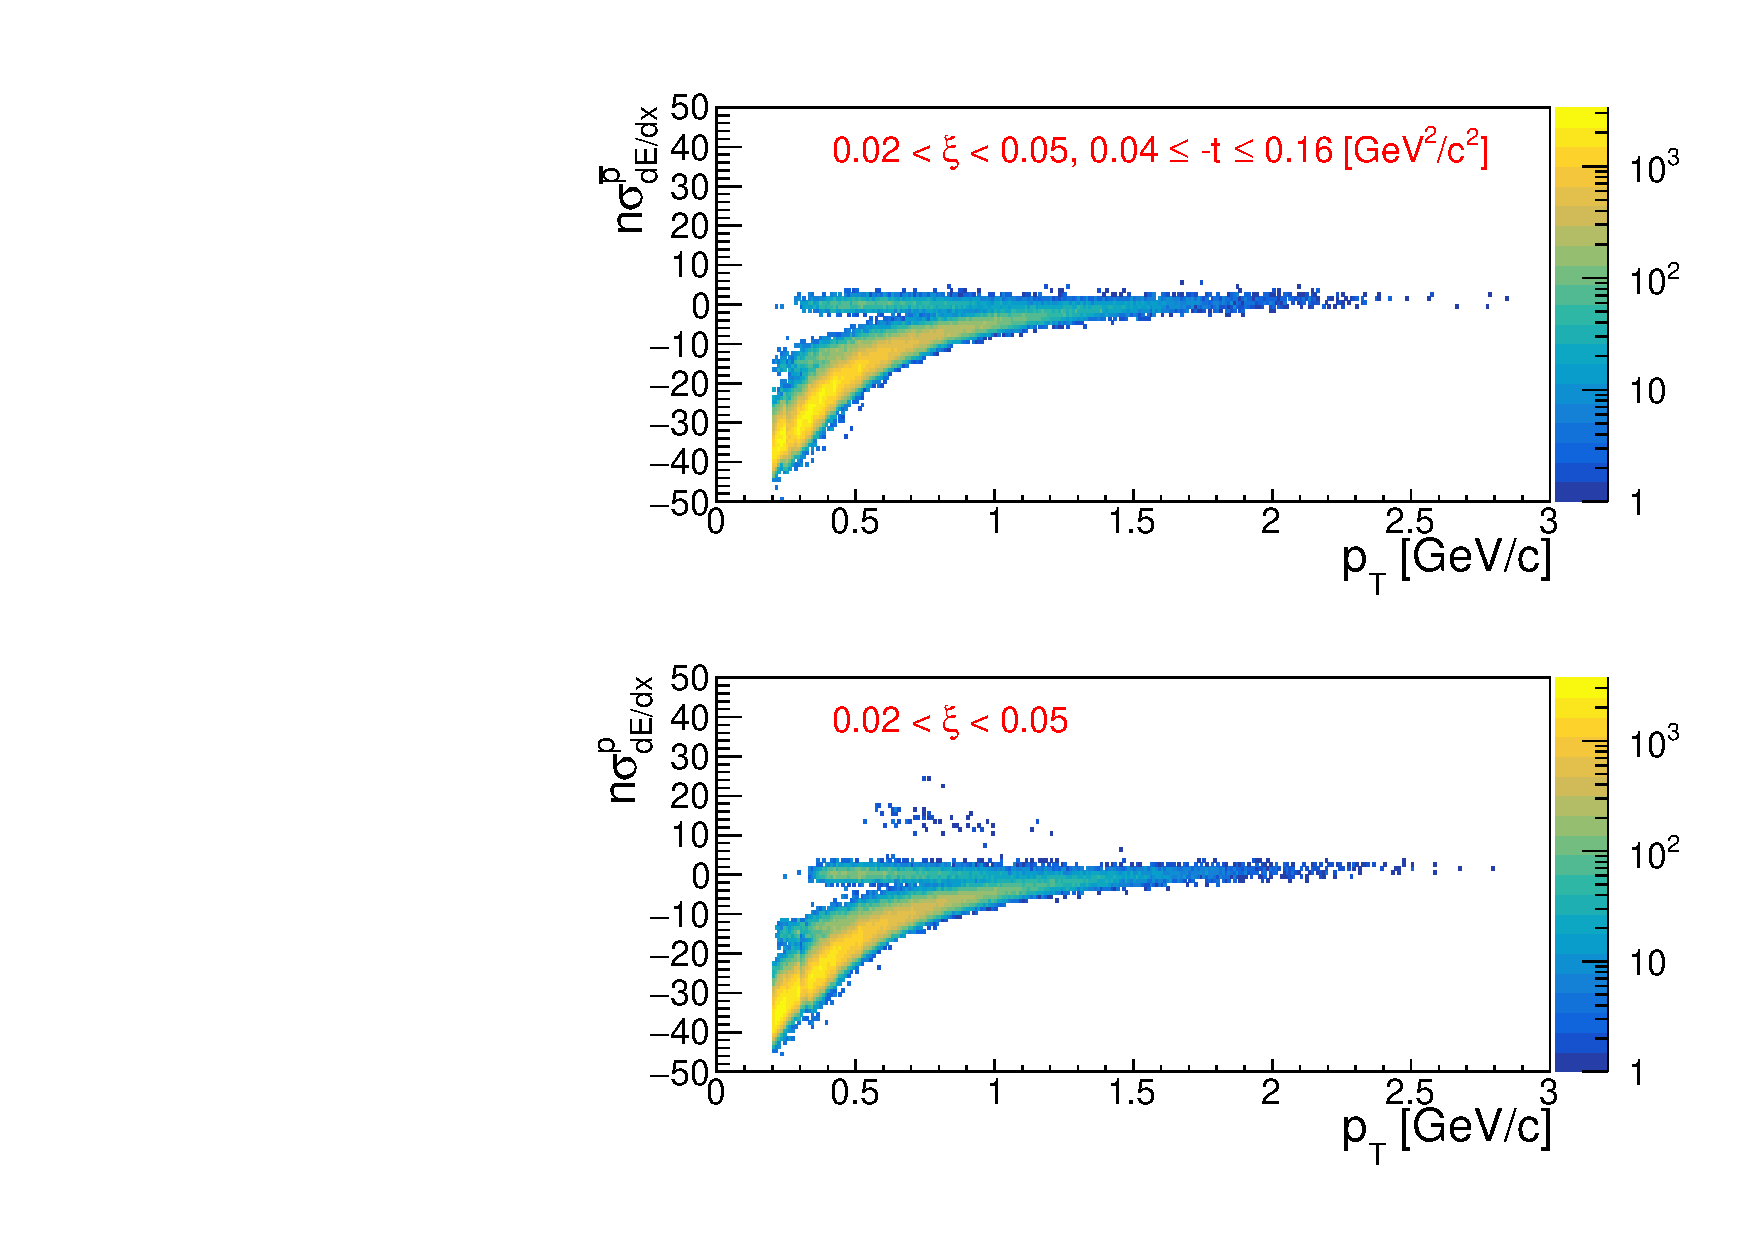
\includegraphics[width=\linewidth, page=1]{chapters/chrgSTAR/img/dEdx/fit2019_2dNsigma_0_2.pdf}
	\end{subfigure}
	\begin{minipage}{.49\textwidth}{The $n\sigma^{i}_{dE/dx}$ variable for particle $i^\pm$ versus $p_\textrm{T}$. Particles are restricted in $|\eta| < 0.7$ and corrected for the energy loss (mass of $i^\pm$-particle was taken)~\cite{supplementaryNote} and vertexing.}
		
	\end{minipage}
	
\end{figure}

\begin{figure}[h!]
	\centering
	\begin{subfigure}{.49\textwidth}
		\includegraphics[width=\linewidth, page=9]{chapters/chrgSTAR/img/dEdx/fit2019_secondStep_0_0.pdf}
	\end{subfigure}
	\begin{subfigure}{.49\textwidth}
		\includegraphics[width=\linewidth, page=7]{chapters/chrgSTAR/img/dEdx/fit2019_thirdStep_1_0.pdf}
	\end{subfigure}\par
	\begin{subfigure}{.49\textwidth}
		\includegraphics[width=\linewidth, page=5]{chapters/chrgSTAR/img/dEdx/fit2019_thirdStep_2_0.pdf}
	\end{subfigure}
	\begin{minipage}{.49\textwidth}
		\caption{Distributions of (top left) $n\sigma^{\pi^\pm}_{dE/dx}$ for $\pi^\pm$, (top right) $n\sigma^{K^\pm}_{dE/dx}$ for $K^\pm$ and (bottom left) $n\sigma^{\bar{p}/p}_{dE/dx}$ for $\bar{p}/p$ in sample  $p_\textrm{T}$ bin and sample $\xi$ range  shown for each particle species. Particles are corrected for  energy loss~\cite{supplementaryNote} and vertexing. The curves represent the Gaussian fits to the $n\sigma^{i}_{dE/dx}$ distributions.}
		\label{fig:dEdx_fit_example}
	\end{minipage}
	
\end{figure}


\noindent Figure \ref{fig:dEdx_fit_example}
shows the $n\sigma^{\pi^\pm}_{dE/dx}$,$n\sigma^{K^\pm}_{dE/dx}$ and $n\sigma^{p(\bar{p})}_{dE/dx}$ distributions for a single $p_\textrm{T}$ bin in the~single $\xi$ range, $0.02 < \xi < 0.05$, each corrected for the energy loss (mass of $i$-particle was assumed)~\cite{supplementaryNote} and vertexing (other $p_\textrm{T}$ bins are shown in Appendix~\ref{appendix:dEdxFits}). To extract the  particle yield for a given particle type,
a~multi-Gaussian fit is applied to the $n\sigma^i_{dE/dx}$ distribution in each $p_\textrm{T}$ bin and $\xi$ range. The parameters of the multi-Gaussian fit are the centroids $\mu_{i^-/i^+}$, widths $\sigma_{i^-/i^+}$, sum  and ratios  of amplitudes $C_{i^-/i^+}$, $r_{i^-/i^+}$ for negative $i^-$ and positive $i^+$ particles ($\pi^\pm$, $e^\pm$, $K^\pm$, $p$ and $\bar{p}$). The positive and negative particle
$n\sigma^{i}_{dE/dx}$-distributions are fit simultaneously, where the particle
and antiparticle centroids and widths are kept the same. Additionally, multiple steps of fitting in the first $\xi$ range are performed to reduce the number of free parameters in the final fit, where almost all centroids and widths are constrained  by an arbitrary function with free parameters $p_k$, where $k \in \mathbb N$. The values of these parameters, obtained for events with $0.02 < \xi < 0.05$ are kept the same for other $\xi$ ranges.
 Also electron contributions are  fixed, but separately for each $\xi$ range. The procedure slightly differs for different particle types:
\begin{enumerate}
	\item  $\pi^{\pm}$:
		\begin{itemize}
			\item Step 1 (Fig. ~\ref{fig:dEdx_fit_parametersPi}):
			\begin{itemize}
				\renewcommand\labelitemi{--}
				\item Analyze data with $0.2 < p_\textrm{T} < 0.65$~GeV/c
				\item Fit  $\mu_{\pi^-/\pi^+}$ and $\sigma_{\pi^-/\pi^+}$ as a function of $p_\textrm{T}$ with a polynomial  $p_0p_\textrm{T}^3+p_1p_\textrm{T}^2+p_2p_\textrm{T}+p_3$
				\item Fit $r_{e^-/e^+}$ as a function of $p_\textrm{T}$ with a polynomial $p_0p_\textrm{T}^2+p_1p_\textrm{T}+p_2$
				\item Fit  $C_{e^-/e^+}$, $\mu_{K^-/K^+}$ as a functions of $p_\textrm{T}$ with $p_0\exp\left(p_1p_\textrm{T}\right)+p_2$
				\item Fit  $\mu_{e^-/e^+}$ as a function of $p_\textrm{T}$ with $p_0\exp\left[-\left(p_1p_\textrm{T}\right)^{p_2}\right]$ 
				\item Fit $\sigma_{K^-/K^+}$ as a function of $p_\textrm{T}$, where $0.3<p_\textrm{T}<0.5$~GeV/c, with constant $p_0$ 
				\item Fit  $\mu_{\bar{p}/p}$ and $\sigma_{\bar{p}/p}$ as a function of $p_\textrm{T}$ with $p_0\exp\left(p_1p_\textrm{T}\right)$
			\end{itemize}
			\item Step 2:
				\begin{itemize}
					\renewcommand\labelitemi{--}
					\item $\sigma_{e^-/e^+}$ fixed to $1.2$ and $0.8$ for $0.2<p_\textrm{T}<0.4$ and $0.4<p_\textrm{T}<0.7$, respectively
					\item $\sigma_{K^-/K^+}$ parametrized for $0.3<p_\textrm{T}<0.7$
					\item  The rest parameters from Step 1 are fixed with obtained parametrization: $\mu_{\pi^-/\pi^+}$, $\sigma_{\pi^-/\pi^+}$, , $r_{e^-/e^+}$, $C_{e^-/e^+}$, $\mu_{e^-/e^+}$ , $\mu_{K^-/K^+}$, $\mu_{\bar{p}/p}$, $\sigma_{\bar{p}/p}$
				\end{itemize}	
		\end{itemize}		
\end{enumerate} 

\begin{enumerate}
	\item[2.] $K^\pm$:
	\begin{itemize}
		\item Step 1 (Fig. ~\ref{fig:dEdx_fit_parametersK}):
		\begin{itemize}
			\renewcommand\labelitemi{--}
			\item Analyze data with $0.2 < p_\textrm{T} < 0.6$~GeV/c
			\item Fit  $\mu_{\pi^-/\pi^+}$  as a function of $p_\textrm{T}$ with $-\exp\left(p_0+p_1p_\textrm{T}\right)$
			\item Fit $\sigma_{\pi^-/\pi^+}$, $C_{e^-/e^+}$, $\sigma_{e^-/e^+}$, $\sigma_{K^-/K^+}$ as a function of $p_\textrm{T}$ with $\exp\left(p_0+p_1p_\textrm{T}\right)$
			\item Fit $r_{e^-/e^+}$ as a function of $p_\textrm{T}$ with constant $p_0$ 
			\item Fit $\mu_{e^-/e^+}$ as a function of $p_\textrm{T}$ with a~polynomial  $p_0p_\textrm{T}^3+p_1p_\textrm{T}^2+p_2p_\textrm{T}+p_3$
			\item Fit $\mu_{K^-/K^+}$ as a function of $p_\textrm{T}$ with a~polynomial  $p_0+p_1p_\textrm{T}^2$
			
		\end{itemize}
		\item Step 2:
		\begin{itemize}
			\renewcommand\labelitemi{--}
			\item All parameters from Step 1 except $\sigma_{e^-/e^+}$ are fixed with obtained parametrization.
			\item  Fit $\sigma_{e^-/e^+}$ as a function of $p_\textrm{T}$, where $0.45<p_\textrm{T}<0.65$~GeV/c, with constant $p_0$ 
			
		\end{itemize}
		\item Step 3:
		\begin{itemize}
			\renewcommand\labelitemi{--}
			\item  $\sigma_{e^-/e^+}$ fixed with obtained parametrization from Steps 1 and 2 for $0.3<p_\textrm{T}<0.45$ and $0.45<p_\textrm{T}<0.65$, respectively.
			\item  The rest parameters from Step 1 are fixed with obtained parametrization: $\mu_{\pi^-/\pi^+}$, $\sigma_{\pi^-/\pi^+}$, , $r_{e^-/e^+}$, $C_{e^-/e^+}$, $\mu_{e^-/e^+}$ , $\mu_{K^-/K^+}$,$\sigma_{K^-/K^+}$
		\end{itemize}		
	\end{itemize}		
\end{enumerate} 

\begin{figure}[h!]
	\centering
	\begin{subfigure}{.32\textwidth}
		\includegraphics[width=\linewidth, page=3]{chapters/chrgSTAR/img/dEdx/fit2019_fitResult_0_0_step_0.pdf}
	\end{subfigure}
	\begin{subfigure}{.32\textwidth}
		\includegraphics[width=\linewidth, page=4]{chapters/chrgSTAR/img/dEdx/fit2019_fitResult_0_0_step_0.pdf}
	\end{subfigure}
	\begin{subfigure}{.32\textwidth}
		\includegraphics[width=\linewidth, page=5]{chapters/chrgSTAR/img/dEdx/fit2019_fitResult_0_0_step_0.pdf}
	\end{subfigure}
	\begin{subfigure}{.32\textwidth}
		\includegraphics[width=\linewidth, page=6]{chapters/chrgSTAR/img/dEdx/fit2019_fitResult_0_0_step_0.pdf}
	\end{subfigure}
	\begin{subfigure}{.32\textwidth}
		\includegraphics[width=\linewidth, page=7]{chapters/chrgSTAR/img/dEdx/fit2019_fitResult_0_0_step_0.pdf}
	\end{subfigure}
	\begin{subfigure}{.32\textwidth}
		\includegraphics[width=\linewidth, page=8]{chapters/chrgSTAR/img/dEdx/fit2019_fitResult_0_0_step_0.pdf}
	\end{subfigure}
	\begin{subfigure}{.32\textwidth}
		\includegraphics[width=\linewidth, page=11]{chapters/chrgSTAR/img/dEdx/fit2019_fitResult_0_0_step_0.pdf}
	\end{subfigure}
	\begin{subfigure}{.32\textwidth}
		\includegraphics[width=\linewidth, page=12]{chapters/chrgSTAR/img/dEdx/fit2019_fitResult_0_0_step_0.pdf}
	\end{subfigure}
	\begin{subfigure}{.32\textwidth}
		\includegraphics[width=\linewidth, page=15]{chapters/chrgSTAR/img/dEdx/fit2019_fitResult_0_0_step_0.pdf}
	\end{subfigure}
	\begin{subfigure}{.32\textwidth}
		\includegraphics[width=\linewidth, page=16]{chapters/chrgSTAR/img/dEdx/fit2019_fitResult_0_0_step_0.pdf}
	\end{subfigure}
	\begin{minipage}{.64\textwidth}
		\caption{Means, widths and electron amplitudes of each $n\sigma^{\pi^\pm}_{dE/dx}$ fit as a function of $p_\textrm{T}$.  The red line on each plot is a~fit function to stabilize and constrain the Gaussian fit parameters for the final fitting step.}
		\label{fig:dEdx_fit_parametersPi}
	\end{minipage}
	
\end{figure}
\begin{enumerate}
	\item[3.] $\bar{p},p$:
	\begin{itemize}
		\item Step 1 (Fig. ~\ref{fig:dEdx_fit_parameters_P}):
		\begin{itemize}
			\renewcommand\labelitemi{--}
			\item Analyze data with $0.4 < p_\textrm{T} < 0.9$~GeV/c
			\item Fit  $\mu_{\pi^-/\pi^+}$, $\mu_{K^-/K^+}$   as a function of $p_\textrm{T}$ with a~polynomial  $p_0p_\textrm{T}+p_1$ 
			\item Fit  $\sigma_{\pi^-/\pi^+}$  as a function of $p_\textrm{T}$ with a~polynomial $p_0p_\textrm{T}^2+p_1p_\textrm{T}+p_2$ 
			\item Fit $\sigma_{K^-/K^+}$ as a function of $p_\textrm{T}$ with $\exp\left(p_0+p_1p_\textrm{T}\right)$
		\end{itemize}
		\item Step 2:
		\begin{itemize}
			\renewcommand\labelitemi{--}
			\item $\mu_{K^-/K^+}$ fixed with obtained parametrization from Step 1
			\item All the rest parameters from Step 1 are limited with obtained parametrization
			\item Fit  $\mu_{\pi^-/\pi^+}$, $\sigma_{\pi^-/\pi^+}$, $\sigma_{K^-/K^+}$  as a function of $p_\textrm{T}$ with a~polynomial $p_0p_\textrm{T}^2+p_1p_\textrm{T}+p_2$ 
			\item Fit  $\mu_{\bar{p}/p}$  as a function of $p_\textrm{T}$, where $0.7<p_\textrm{T}<1.0$~GeV/c, with constant $p_0$ 
			
		\end{itemize}
		\item Step 3:
		\begin{itemize}
			\renewcommand\labelitemi{--}
			\item  $\mu_{K^-/K^+}$ fixed with obtained parametrization from Step 1
			\item $\mu_{\bar{p}/p}$  fixed with obtained parametrization from Step 2 for $0.7<p_\textrm{T}<1.0$
			\item  The rest parameters from Step 2 are fixed with obtained parametrization: $\mu_{\pi^-/\pi^+}$, $\sigma_{\pi^-/\pi^+}$, $\sigma_{K^-/K^+}$
		\end{itemize}		
	\end{itemize}		
\end{enumerate} 


\begin{figure}[h!]
	\centering
	\begin{subfigure}{.32\textwidth}
		\includegraphics[width=\linewidth, page=3]{chapters/chrgSTAR/img/dEdx/fit2019_fitResult_2_0_step_1.pdf}
	\end{subfigure}
	\begin{subfigure}{.32\textwidth}
		\includegraphics[width=\linewidth, page=4]{chapters/chrgSTAR/img/dEdx/fit2019_fitResult_2_0_step_1.pdf}
	\end{subfigure}
	\begin{subfigure}{.32\textwidth}
		\includegraphics[width=\linewidth, page=11]{chapters/chrgSTAR/img/dEdx/fit2019_fitResult_2_0_step_0.pdf}%done
	\end{subfigure}
	\begin{subfigure}{.32\textwidth}
		\includegraphics[width=\linewidth, page=12]{chapters/chrgSTAR/img/dEdx/fit2019_fitResult_2_0_step_1.pdf}
	\end{subfigure}
		\begin{subfigure}{.32\textwidth}
			\includegraphics[width=\linewidth, page=15]{chapters/chrgSTAR/img/dEdx/fit2019_fitResult_2_0_step_1.pdf}
		\end{subfigure}
	\caption{Means and widths  of each $n\sigma^{\bar{p}/p}_{dE/dx}$ fit as a function of $p_\textrm{T}$.  The red line on each plot is a~fit function to stabilize and constrain the Gaussian fit parameters for the final fitting step.}
	\label{fig:dEdx_fit_parameters_P}
	
\end{figure}
\begin{figure}[h!]
	\centering
	\begin{subfigure}{.32\textwidth}
		\includegraphics[width=\linewidth, page=3]{chapters/chrgSTAR/img/dEdx/fit2019_fitResult_1_0_step_0.pdf}
	\end{subfigure}
	\begin{subfigure}{.32\textwidth}
		\includegraphics[width=\linewidth, page=4]{chapters/chrgSTAR/img/dEdx/fit2019_fitResult_1_0_step_0.pdf}
	\end{subfigure}
	\begin{subfigure}{.32\textwidth}
		\includegraphics[width=\linewidth, page=5]{chapters/chrgSTAR/img/dEdx/fit2019_fitResult_1_0_step_0.pdf}
	\end{subfigure}
	\begin{subfigure}{.32\textwidth}
		\includegraphics[width=\linewidth, page=6]{chapters/chrgSTAR/img/dEdx/fit2019_fitResult_1_0_step_0.pdf}
	\end{subfigure}
	\begin{subfigure}{.32\textwidth}
		\includegraphics[width=\linewidth, page=7]{chapters/chrgSTAR/img/dEdx/fit2019_fitResult_1_0_step_0.pdf}
	\end{subfigure}
	\begin{subfigure}{.32\textwidth}
		\includegraphics[width=\linewidth, page=8]{chapters/chrgSTAR/img/dEdx/fit2019_fitResult_1_0_step_0.pdf}
	\end{subfigure}
	\begin{subfigure}{.32\textwidth}
		\includegraphics[width=\linewidth, page=11]{chapters/chrgSTAR/img/dEdx/fit2019_fitResult_1_0_step_0.pdf}
	\end{subfigure}
	\begin{subfigure}{.32\textwidth}
		\includegraphics[width=\linewidth, page=12]{chapters/chrgSTAR/img/dEdx/fit2019_fitResult_1_0_step_0.pdf}
	\end{subfigure}
	\caption{Means, widths and electron amplitudes of each $n\sigma^{K^\pm}_{dE/dx}$ fit as a function of $p_\textrm{T}$.  The red line on each plot is a~fit function to stabilize and constrain the Gaussian fit parameters for the final fitting step.}
	\label{fig:dEdx_fit_parametersK}
	%\vspace{-2cm}
\end{figure}

The particle yield is extracted from the fit to the corresponding
$n\sigma^{i}_{dE/dx}$  distribution (corrected only for the energy loss~\cite{supplementaryNote} and vertexing). As shown in Fig.~\ref{fig:dEdx_nsigma}, the $dE/dx$ of each particle type merge at large $p_\textrm{T}$. Hence, the particle identification is limited. Pions can be identified
in the momentum range of $0.2-0.7$~GeV/c, kaons in
$0.3-0.65$~GeV/c and (anti)protons in $0.4-1.0$~GeV/c. 
%\FloatBarrier
